% Final wrapper for Chapter 3. The v8 text is the audited semantic source of truth.
\begingroup
\newcount\ThesisChThreeSubsec
\newcount\ThesisChThreeSubsub
\ThesisChThreeSubsec=0
\ThesisChThreeSubsub=0
\let\ThesisChThreeOriginalSubsection\subsection
\let\ThesisChThreeOriginalSubsubsection\subsubsection
\renewcommand{\subsection}[1]{%
  \advance\ThesisChThreeSubsec by 1%
  \ifnum\ThesisChThreeSubsec=5
    \begin{figure}[htbp]
      \centering
      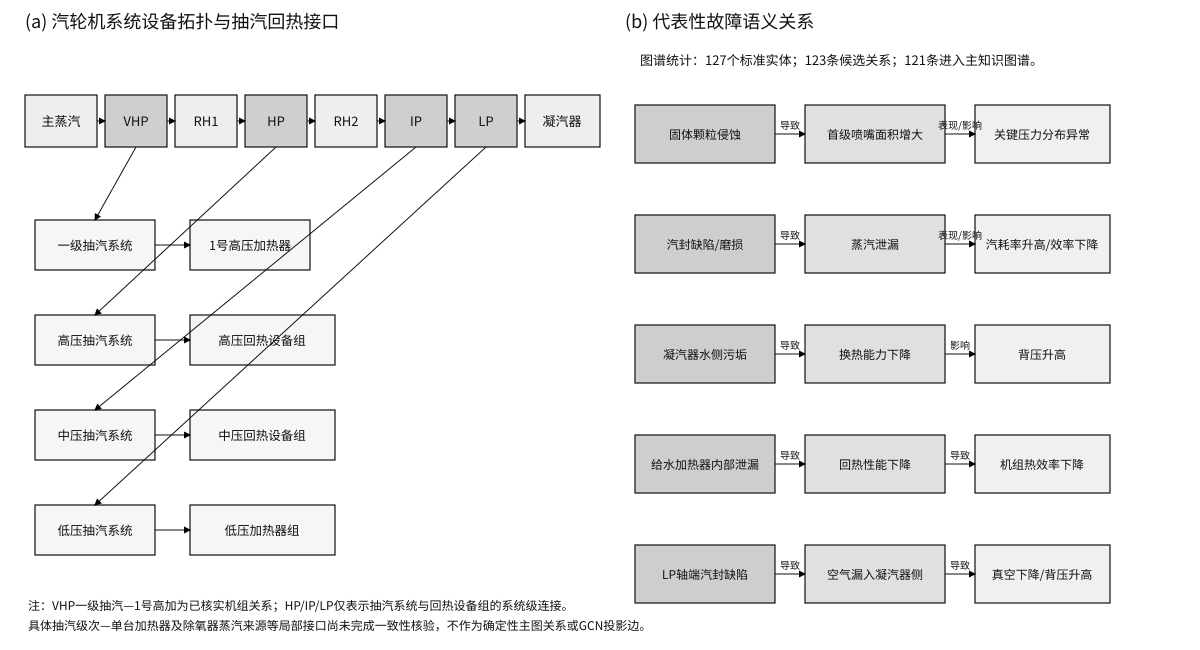
\includegraphics[width=0.99\textwidth]{figures/ch3/fig3_2_turbine_kg_overview.pdf}
      \caption{汽轮机系统知识图谱设备拓扑及代表性故障语义关系}
      \label{fig:turbine_kg_overview_final}
    \end{figure}
    图~\ref{fig:turbine_kg_overview_final}仅展示进入主知识图谱的可审计设备拓扑及代表性故障语义链路，用于说明系统结构与故障知识的组织方式；完整关系仍以审查后的知识三元组为准。存在资料差异的候选接口保持待核状态，不作为确定性图关系或后续GCN投影边。
  \fi
  \ThesisChThreeOriginalSubsection{#1}%
}
\renewcommand{\subsubsection}[1]{%
  \advance\ThesisChThreeSubsub by 1%
  \ifnum\ThesisChThreeSubsub=2
    \begin{figure}[htbp]
      \centering
      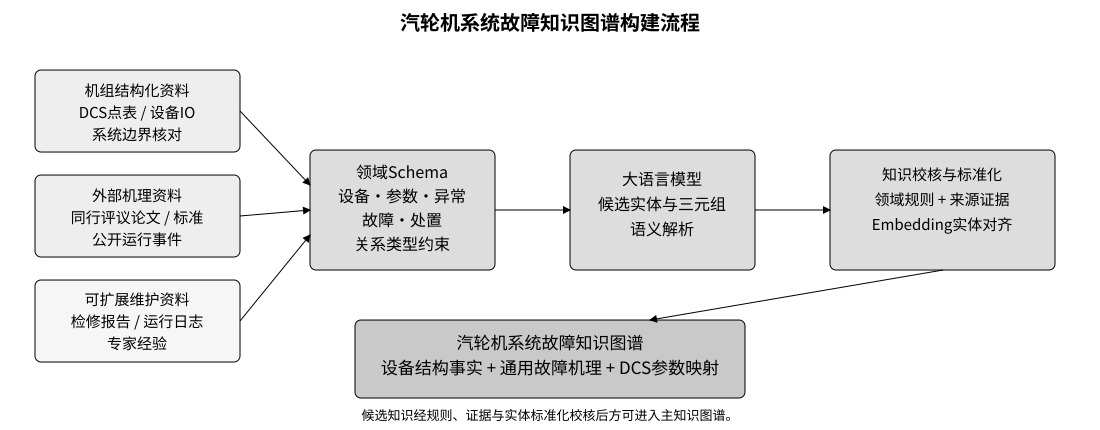
\includegraphics[width=0.98\textwidth]{figures/ch3/fig3_1_kg_construction_flow.pdf}
      \caption{汽轮机系统故障知识图谱构建流程}
      \label{fig:kg_construction_flow_final}
    \end{figure}
  \fi
  \ThesisChThreeOriginalSubsubsection{#1}%
}
\section{基于运行生产资料的汽轮机系统故障知识图谱构建}
\label{sec:knowledge_graph_v8}

\subsection{引言}

燃煤机组汽轮机系统由多级汽缸、再热系统、抽汽回热系统以及凝汽器冷端等多个热力设备组成，各设备通过蒸汽、凝结水和给水持续进行物质与能量传递。局部设备发生通流、汽封或换热性能异常后，其影响通常不会局限于单一监测参数，而会沿实际热力连接向相邻设备和参数传播。第二章建立的健康状态模型能够在给定运行边界下获得设备状态参数的健康参考值，并由实测值与模型输出之间的偏差信息表征状态变化程度。然而，仅依据参数偏差仍难以刻画参数所属设备、参数之间的物理联系以及多参数异常与故障机理之间的关联。

电站长期设计、运行和维护过程中积累了大量设备结构、DCS测点、系统接口、故障分析和检修经验等生产资料。这些知识既存在于点表、设备清单等结构化数据中，也分布于技术报告、标准和公开文献等文本资料中。知识图谱（Knowledge Graph，KG）能够以实体和关系组织多源异构知识，并利用图结构显式表示设备、参数、异常与故障之间的语义联系\cite{Hogan2021KnowledgeGraphs}。因此，将汽轮机运行生产资料转化为领域知识图谱，可以为后续图卷积故障诊断提供具有工程含义的结构先验。

本章首先分析汽轮机系统参数关联与典型故障特性，明确知识图谱需要描述的对象；随后整理机组DCS点表、设备输入输出关系和系统边界资料，并利用公开论文、标准及运行事件资料补充故障机理知识；在此基础上定义实体和关系类型，采用大语言模型生成候选三元组，并通过领域规则、来源证据和Embedding语义对齐完成知识校核与实体标准化。最终形成能够与实际DCS状态量建立映射的汽轮机系统故障知识图谱。

\subsection{燃煤机组汽轮机系统参数及故障特性}
\label{subsec:turbine_fault_characteristics_v8}

汽轮机主通流可概括为“主蒸汽--VHP--一次再热--HP--二次再热--IP--LP--凝汽器”。主蒸汽压力、温度和流量构成VHP入口热力边界，VHP排汽进入一次再热系统，一次热再蒸汽形成HP入口条件，HP排汽经二次再热后进入IP，最终蒸汽经LP膨胀后排入凝汽器。除主通流外，各级汽缸还通过抽汽支路向回热系统提供热源，使汽轮机本体与高压加热器、低压加热器、除氧器及给水系统形成进一步耦合。

根据已核对的机组资料，VHP一级抽汽与1号高压加热器相连。对于HP、IP和LP侧回热支路，现有资料能够确认其分别通过高压、中压和低压抽汽系统与相应回热设备形成系统级连接，但对具体抽汽级次与单台加热器的一一对应尚未完成机组级一致性核验；除氧器蒸汽来源等局部接口在不同资料中亦存在差异。因此，本文系统级知识图谱仅保留已核实的VHP一级抽汽--1号高压加热器关系，以及HP、IP、LP与相应抽汽/回热设备组之间的系统级连接，不将尚未核实的具体级次--单台设备关系作为确定性拓扑写入后续参数图。

汽轮机热力故障通常表现为多个状态参数的协同变化。Kubiak等针对汽轮机部件退化的案例研究表明，固体颗粒侵蚀会改变喷嘴或叶片有效通流面积，并影响关键压力分布\cite{Kubiak2002TurbineDegradation}。针对蒸汽轮机叶片沉积的跨型式研究进一步表明，沉积可减小有效通流面积，并可能降低出力和效率\cite{Kubiak2002ScaleDeposit}。该研究对象为地热蒸汽轮机，因此本文仅将其作为通用蒸汽轮机沉积机理参考，而不作为本文燃煤机组的现场直接证据。

汽封异常同样具有明显的结构传播特征。级间或轴端汽封缺陷会增加蒸汽泄漏，并影响汽轮机经济性；低压侧轴端密封异常还可能造成空气漏入和真空损失\cite{ZhangHu2021FaultPropagationGNN}。针对HP--IP中间汽封泄漏的研究表明，热再温度、IP排汽温度以及IP效率与该类泄漏具有诊断关联\cite{Xu2011HPIPLeakage}。上述关系反映的是设备层面和参数层面的通用机理，不直接规定本文VHP某一具体DCS测点的固定增减方向。

冷端和回热系统的故障也会沿热力接口影响汽轮机状态。燃煤机组凝汽器研究表明，水侧污垢会降低凝汽器换热有效性；凝汽压力还受到循环水温度、流量及换热状态等因素影响，并进一步影响机组热力性能\cite{Li2016CondenserFouling,Medica2018CondenserCondition}。给水加热器内部泄漏会破坏正常回热过程并影响循环效率，换热功率等过程指标可用于跟踪加热器慢性性能变化\cite{Heo2012FWHLeakage,Barszcz2011FeedwaterHeater}。

由上述过程可见，同一故障在多个参数上的响应受到设备归属和热力传播路径约束，而不同故障又可能共享部分压力、温度或流量参数。若仅依据局部数值相似性进行分类，容易产生故障类别混淆。因此，故障知识图谱需要同时表示设备连接、参数归属、故障发生位置、异常表现及处置关系，为多参数故障诊断提供结构化知识基础。

\subsection{基于运行生产资料的知识图谱构建方法}
\label{subsec:kg_construction_v8}

\subsubsection{汽轮机热力过程的运行生产资料}
\label{subsubsec:operation_materials_v8}

运行生产资料是领域故障知识图谱的主要知识来源。本文能够直接获得的机组资料包括DCS测点表、设备输入输出关系、系统边界核对结果以及状态监测建模资料。该类资料主要用于确定设备名称、参数点号、参数归属、主通流方向、抽汽支路及相邻设备接口，为设备实体、参数实体和机组拓扑关系提供事实依据。

现场结构资料难以完整覆盖典型故障的原因、演化过程和异常表现。为补充故障机理知识，本文进一步引入同行评议论文、标准、设备运行维护资料和公开运行事件报告。跨机组资料主要用于提取具有通用物理意义的“故障--异常--参数”关系，不直接将其他机组中某一具体测点的变化方向套用于本文机组。主要资料来源及用途见表~\ref{tab:kg_sources_v8}。

\begin{table}[htbp]
    \centering
    \caption{汽轮机故障知识图谱的主要知识来源}
    \label{tab:kg_sources_v8}
    \begin{tabular}{p{3.8cm}p{5.2cm}p{5.2cm}}
        \toprule
        资料类型 & 主要内容 & 图谱中的主要用途 \\
        \midrule
        DCS点表与设备IO资料 & 测点名称、点号、设备归属、入口和出口边界 & 构建设备、参数实体及机组直接拓扑 \\
        系统边界与状态建模资料 & 主通流、抽汽、再热及设备边界关系 & 校核设备接口和DCS映射 \\
        同行评议论文 & 汽封泄漏、通流侵蚀、沉积、冷端及回热故障机理 & 提取故障、异常和参数之间的通用关系 \\
        标准、维护资料及公开运行事件 & 故障现象、运行影响和处置经验 & 补充并交叉核验故障关系 \\
        \bottomrule
    \end{tabular}
\end{table}

在知识入图过程中，对机组结构事实与外部故障机理进行分层管理。由DCS、设备IO和系统拓扑直接确认的关系用于描述本文机组设备结构；由论文、标准或公开运行事件直接支持的关系用于描述通用故障机理；仅能依据热力规律推导而缺少直接证据的点级响应不作为主知识图谱中的确定关系。这样既保持机组拓扑与实际对象一致，也避免将跨机组经验过度外推至具体DCS测点。

\begin{figure}[htbp]
    \centering
    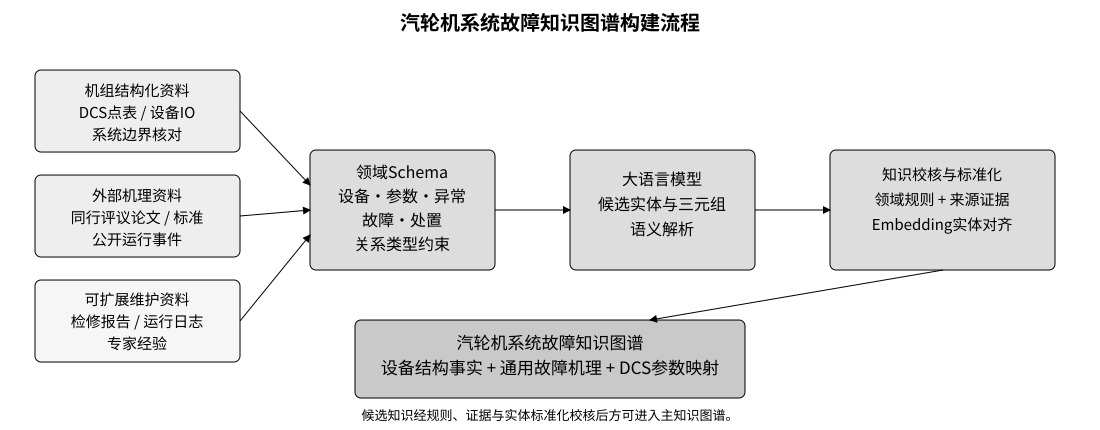
\includegraphics[width=0.98\textwidth]{figures/ch3/fig3_1_kg_construction_flow.pdf}
    \caption{汽轮机系统故障知识图谱构建流程}
    \label{fig:kg_construction_flow_v8}
\end{figure}

\subsubsection{节点和关系的构建与提取}
\label{subsubsec:entity_relation_v8}

运行生产资料中的设备、参数和故障信息通常以自然语言、工程简称或DCS编码等不同形式出现，同一对象在不同资料中可能存在多种表达。若缺少统一的实体和关系定义，知识抽取结果容易出现实体重复、语义边界不清以及关系方向混杂等问题。因此，首先需要建立适用于汽轮机故障诊断的知识图谱Schema。

设汽轮机系统故障知识图谱为
\begin{equation}
G_{KG}=(V,E,\mathcal R),
\end{equation}
式中：$V$为实体集合；$E$为实体间关系边集合；$\mathcal R$为关系类型集合。根据诊断任务需求，将实体划分为设备、参数、异常、故障和处置五类：
\begin{equation}
V=V_{dev}\cup V_{par}\cup V_{abn}\cup V_{fault}\cup V_{act}.
\end{equation}
设备实体表示VHP、HP、IP、LP、再热系统、抽汽支路、加热器和凝汽器等物理对象；参数实体表示可由DCS直接获取的压力、温度、流量和阀位等运行量；异常实体描述蒸汽泄漏、真空下降、通流面积变化和效率降低等状态现象；故障实体表示具有独立工程含义的故障类型；处置实体表示检查、清洗和检修等维护措施。

在实体类型确定后，根据汽轮机系统结构和故障语义定义设备归属、介质流向、设备接口、发生于、导致、表现为、影响、关联监测和处置为等关系。主要关系类型见表~\ref{tab:kg_relation_types_v8}。

\begin{table}[htbp]
    \centering
    \caption{汽轮机故障知识图谱主要关系类型}
    \label{tab:kg_relation_types_v8}
    \begin{tabular}{lll}
        \toprule
        关系类型 & 头实体类型 & 尾实体类型 \\
        \midrule
        归属 & 参数 & 设备 \\
        介质流向/设备接口 & 设备 & 设备 \\
        发生于 & 故障 & 设备 \\
        导致/表现为 & 故障或异常 & 异常 \\
        影响/关联监测 & 故障或异常 & 参数 \\
        处置为 & 故障 & 处置 \\
        \bottomrule
    \end{tabular}
\end{table}

完成Schema定义后，利用大语言模型对设备资料和故障文本进行语义解析，并按照预定义实体与关系类型输出候选三元组。语言模型能够快速识别文本中的设备、参数、异常、故障及处置对象，但其输出仅作为候选知识，不能直接写入最终图谱。

候选三元组首先经过领域规则校核。规则包括实体类型约束、关系方向约束、设备兼容性约束和参数可观测性约束。例如，“压力升高”“阀位异常”等带有状态方向的表达应归入异常实体，而不能作为实时数值参数节点；不存在于本文机组结构中的设备连接，也不能仅依据通用汽轮机结构建立为机组确定关系。通过规则校核可剔除类型错误、方向错误和设备不兼容的候选知识。

经过规则校核后，再对实体名称进行标准化。本文采用Embedding语义对齐处理设备简称、参数别名和不同文本写法\cite{Reimers2019SentenceBERT}。对于候选实体$v_i$和标准实体$v_j$，综合语义向量相似度和字符串相似度计算匹配程度：
\begin{equation}
S_{ij}=\lambda S_{emb}(v_i,v_j)+(1-\lambda)S_{str}(v_i,v_j),
\end{equation}
式中：$S_{emb}$为Embedding语义相似度；$S_{str}$为字符串相似度；$\lambda$为两类相似度的权重系数。当综合相似度达到设定阈值且实体类型一致时，将候选实体归并至标准实体；否则保留为待核对象。

最后，综合候选抽取、规则校核、实体标准化结果和来源证据评价关系可靠性。对于第$e$条候选关系，其置信度可表示为
\begin{equation}
C_e=\alpha C_{llm}+\beta C_{rule}+\gamma C_{emb}+\delta C_{evi},
\end{equation}
式中：$C_{llm}$为语言模型候选抽取置信度；$C_{rule}$为领域规则一致性得分；$C_{emb}$为实体语义对齐置信度；$C_{evi}$为来源证据强度；$\alpha$、$\beta$、$\gamma$和$\delta$为相应权重。机组设备连接关系以DCS和设备IO资料为优先依据，故障机理关系保留可追溯的论文、标准或运行事件来源。经过上述处理，分散于多源资料中的知识被统一表示为“头实体--关系--尾实体”三元组，并组成汽轮机系统故障知识图谱。

\subsection{知识图谱构建结果}
\label{subsec:kg_result_v8}

按照上述流程，形成了覆盖汽轮机主通流、再热、抽汽回热和凝汽冷端等对象的故障知识库。审查后的知识库共包含127个标准实体和123条候选关系。其中81条关系来自本文机组设备结构与DCS资料，40条关系由公开论文、标准或运行事件中的直接故障机理支撑；另有2条候选关系因不同机组资料之间存在描述差异而暂不纳入主知识图谱。因此，当前用于论文知识表达和后续参数图投影的主知识图谱包含121条可用关系。

在设备拓扑方面，图谱保存“主蒸汽--VHP--一次再热--HP--二次再热--IP--LP--凝汽器”的主通流关系，并包含VHP一级抽汽至1号高压加热器，以及HP、IP、LP与高压、中压、低压抽汽系统及相应回热设备组之间的系统级连接。对具体抽汽级次--单台加热器和除氧器蒸汽来源等尚存在资料差异的局部接口，保持待核状态，不进入确定性参数图。在故障语义方面，图谱进一步连接汽封缺陷、蒸汽泄漏、通流侵蚀、叶片沉积、凝汽器污垢和回热设备泄漏等故障与相应异常状态、关联参数及处置知识。

系统级知识图谱用于表达完整汽轮机故障领域知识，而图卷积模型需要加载可实时获取的数值特征。因此，在知识图谱构建完成后，进一步建立标准参数实体与实际DCS测点之间的映射。第五章VHP代表性算例从系统知识图谱中抽取VHP本体、一级抽汽支路和一次再热接口对应的状态参数节点，形成设备任务参数子图，并将第二章健康状态模型产生的动态偏差信息加载至对应参数节点，实现静态领域知识与动态运行数据之间的连接。

\begin{figure}[htbp]
    \centering
    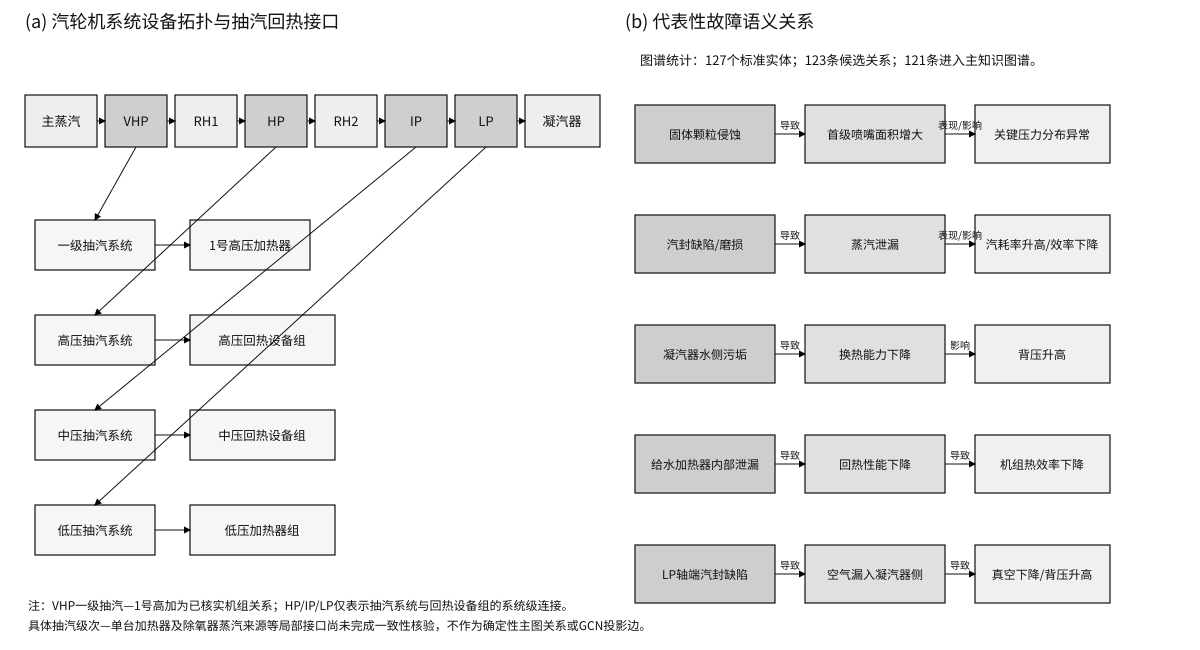
\includegraphics[width=0.99\textwidth]{figures/ch3/fig3_2_turbine_kg_overview.pdf}
    \caption{汽轮机系统知识图谱设备拓扑及代表性故障语义关系}
    \label{fig:turbine_kg_overview_v8}
\end{figure}

图~\ref{fig:turbine_kg_overview_v8}仅展示进入主知识图谱的可审计设备拓扑及代表性故障语义链路。VHP一级抽汽--1号高压加热器为已核实的机组直接关系；HP、IP和LP侧仅表示抽汽系统与相应回热设备组的系统级连接。具体抽汽级次--单台加热器以及除氧器蒸汽来源等尚未完成机组级一致性核验的局部接口，不作为确定性主图关系或后续GCN投影边。

\subsection{本章小结}

本章面向燃煤机组汽轮机系统构建了基于运行生产资料的故障知识图谱。首先分析汽轮机主通流、再热、抽汽回热和凝汽冷端之间的参数关联及典型热力故障的多参数传播特征；随后整理机组DCS点表、设备IO和系统边界资料，并利用公开论文、标准和运行事件补充故障机理知识；在此基础上定义设备、参数、异常、故障和处置等实体及相应关系类型，采用大语言模型生成候选三元组，并结合领域规则、来源证据和Embedding语义对齐完成知识校核与实体标准化。最终形成能够与实际DCS参数建立映射的汽轮机系统故障知识图谱，为下一章基于知识图谱和图卷积网络的故障诊断模型提供静态结构信息。
\endgroup
